%doc: Banc dels aliments/Article Banc aliments.doc
\begin{news}
{2} %columnes
{La nostra escola amb el banc dels aliments}
%index: Banc d'Aliments
{Novament aquest any, l’escola s’ha volgut sumar a la feina que està realitzant el Banc dels Aliments amb una recapta que hem portat a terme la segona quinzena de novembre, després que responsables d’aquesta entitat fessin una xerrada amb l’alumnat de 3r d’ESO}
{Fem Escola}
{101} %pagesof

\noindent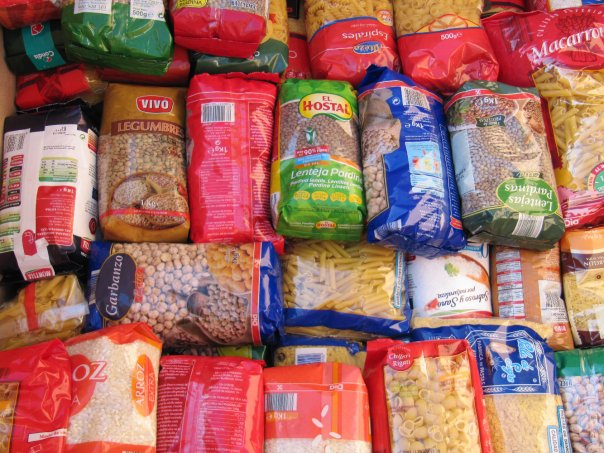
\includegraphics[width=9cm,keepaspectratio]{fem_escola/img/aliments.jpg}

El Banc dels Aliments és una fundació benèfica privada, independent i sense ànim de lucre, que té com a objectiu lluitar contra la fam d’aquí, i evitar que els aliments consumibles però no comercialitzables siguin destruïts i fer-los arribar a les persones més necessitades del nostre entorn immediat.

Tota l’acció del Banc dels Aliments es basa en la gratuïtat dels aliments que reben i de la seva distribució justa a través de les entitats solidàries que atenen els beneficiaris finals. Això es du a terme gràcies al treball d’un grup de més de 100 persones, la gran majoria voluntàries.

En els darrers mesos, les bosses de pobresa i de col·lectius marginats han crescut de forma exponencial i, en conseqüència, la demanda d’aliments que fan les entitats receptores quasi s'ha duplicat.

Paral·lelament, el Banc dels Aliments ha continuat comprovant que en la nostra societat es continuen destruint aliments aprofitables. Tot i que cada vegada les empreses fabricants de productes alimentaris són més conscients que cal evitar aquest malbaratament, als abocadors segueixen arribant aliments que s’haurien pogut aprofitar complint totes les normes sanitàries.

Tothom pot col·laborar amb els Banc dels Aliments: les empreses donant-los els excedents de productes consumibles, les persones fent donacions d’aliments, i tothom ajudant econòmicament o fent de voluntari per tal d'aconseguir més aliments per repartir entre els més necessitats de casa nostra.

Malauradament, la fam ara té més boques. Moltes persones d’aquí es troben en aquesta trista situació i per això cal que els donem un cop de mà.

\end{news}
